\documentclass{article}
\usepackage[utf8]{inputenc}
\usepackage{multicol}
\usepackage[a4paper, left=2cm, right=2cm, top=3cm, bottom=3cm]{geometry}
\usepackage{hyperref}
\usepackage{booktabs}
\usepackage{graphicx}
\usepackage{ragged2e}
\usepackage{graphicx}
\usepackage{float}
\usepackage{hyperref}



\title{Real-time Domain Adaptation in Semantic Segmentation}
\author{Attrovio Mario, Ghisolfo Giorgia, Russo Michele}

\begin{document}
	\maketitle
	
	\begin{multicols}{2}
		
		
		
		\section{Abstract}
		Semantic segmentation is a critical task in computer vision, enabling pixel-wise classification of images. However, the performance of segmentation models often degrades when applied to data from different domains, a challenge known as domain shift. This report explores real-time semantic segmentation in the context of domain adaptation using PIDNet as the backbone. We investigate the performance drop caused by domain shift between urban and rural datasets and evaluate mitigation strategies, including data augmentation and advanced domain adaptation techniques like adversarial training and image-to-image translation (DACS)\cite{tranheden2021dacs}. Experimental results on the LoveDA dataset \cite{loveda2021} demonstrate that these methods reduce the impact of domain shift while maintaining real-time inference capabilities, achieving a balanced trade-off between accuracy and computational efficiency. The code can be found on our project website: \url{https://github.com/MichelePoli/AMLProject}.
		
		\section{Introduction}
		Semantic segmentation is a foundational task in computer vision, where each pixel in an image is assigned a label corresponding to a predefined class. It plays a vital role in applications such as autonomous driving, medical imaging, and remote sensing. Recent advancements in deep learning have yielded high-performing models, but these often struggle with domain shift—a phenomenon where a model trained on a source domain (e.g., urban images) performs poorly on a target domain (e.g., rural images) \cite{loveda2021}. Addressing this challenge is crucial for real-world deployments where annotated data for all target domains is scarce or unavailable.
		
		Domain adaptation aims to bridge this performance gap by aligning the source and target domains without requiring extensive labeled data from the target domain. While several methods exist, real-time semantic segmentation introduces additional constraints, such as maintaining high inference speed and low computational cost. PIDNet \cite{pidnet2023}, a real-time segmentation network inspired by Proportional-Integral-Derivative (PID) controllers, serves as the backbone for our study due to its efficiency and accuracy in real-time tasks.
		
		This report focuses on evaluating and improving the performance of PIDNet for domain-adaptive semantic segmentation using the LoveDA dataset \cite{loveda2021} (Figure \ref{fig:dataset_urban_image1}). We first quantify the performance degradation caused by domain shift. Next, we implement data augmentation techniques and two domain adaptation approaches—adversarial training and image-to-image translation (DACS)\cite{tranheden2021dacs} —to mitigate this issue. Our findings highlight the potential of these methods to enhance generalization while preserving the real-time capabilities of the model.
		
		\begin{figure}[H]
			\centering
			\begin{minipage}{0.48\linewidth}
				\centering
				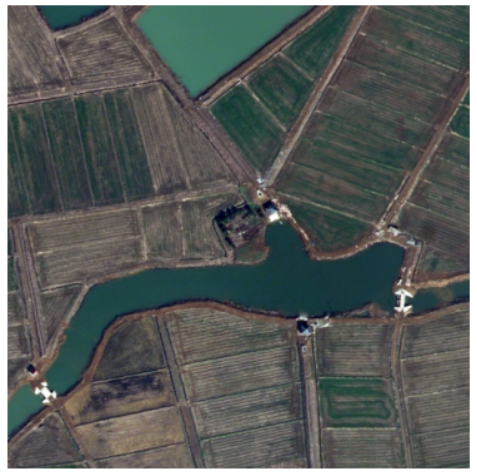
\includegraphics[width=1\linewidth]{image/rural_1.png}

			\end{minipage}
			\begin{minipage}{0.48\linewidth}
				\centering
				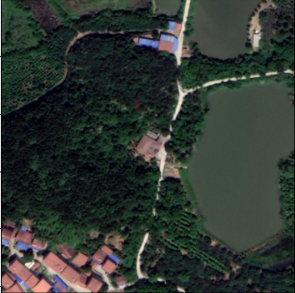
\includegraphics[width=1\linewidth]{image/rural_4.png}
				
			\end{minipage}

			\label{fig:dataset_rural_image1}

			\hfill

			\begin{minipage}{0.48\linewidth}
				\centering
				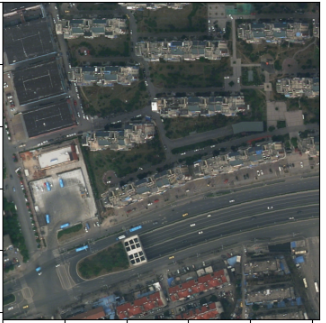
\includegraphics[width=1\linewidth]{image/urban_1.png}

			\end{minipage}
			\begin{minipage}{0.48\linewidth}
				\centering
				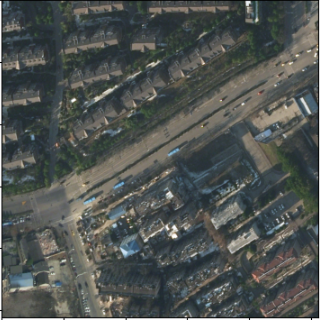
\includegraphics[width=1\linewidth]{image/urban_3.png}

			\end{minipage}

			\caption{Satellite imagery: (Top) Rural images, (Bottom) urban images }
			\label{fig:dataset_urban_image1}

		\end{figure}

	\end{multicols}


	\begin{figure}[H]
		\centering
		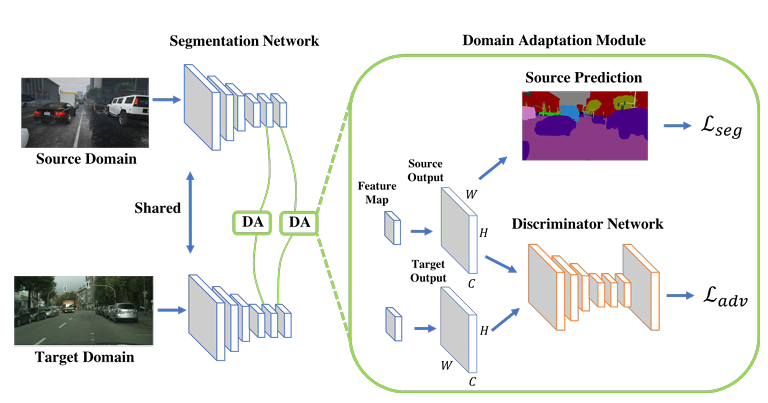
\includegraphics[width=0.7\linewidth]{image/general/adversarial_model.png}
		\caption{Algorithmic overview. Given images with the size H by W in source and target domains, we pass them through the segmentation
		network to obtain output predictions. For source predictions with C categories, a segmentation loss is computed based on the source ground
		truth. To make target predictions closer to the source ones, we utilize a discriminator to distinguish whether the input is from the source or
		target domain. Then an adversarial loss is calculated on the target prediction and is back-propagated to the segmentation network. We call
		this process as one adaptation module, and we illustrate our proposed multi-level adversarial learning by adopting two adaptation modules
		at two different levels here.}
		\label{fig:adversarial_model}
	\end{figure}
	
	\begin{multicols}{2}


		\section{Related work}
		Semantic segmentation has evolved significantly with deep learning. 
		\\
		\\
		\textbf{Foundational architectures}
		Semantic segmentation's deep learning era began with the introduction of Fully Convolutional Networks (FCNs) \cite{long2015fcn}. By replacing fully connected layers with convolutional ones, FCNs enabled end-to-end segmentation, capable of handling images of arbitrary sizes and providing pixel-wise predictions. This innovation laid the groundwork for modern segmentation models.
		Further advancements were introduced with DeepLabV2 \cite{chen2018deeplab}, which leveraged atrous (or dilated) convolutions. Atrous convolutions expanded the receptive field without increasing the number of parameters, making it possible to aggregate multi-scale contextual information efficiently.
		\\




		\textbf{Real-time efficiency}
		Real-time semantic segmentation requires optimizing the balance between accuracy and computational efficiency. BiSeNet \cite{yu2018bisenet} introduced lightweight backbones and parallel structures, achieving an effective speed-accuracy trade-off. This architecture focused on enhancing real-time processing capabilities for applications with strict latency requirements. PIDNet \cite{pidnet2023} further pushed the boundaries of efficiency by adopting principles from PID (Proportional-Integral-Derivative) controllers. The model effectively balanced high-, mid-, and low-level features, offering improvements in both speed and segmentation quality.
		
		\textbf{Domain adaptation techniques}
		Semantic segmentation models often suffer performance degradation when applied across different domains (e.g., urban vs. rural settings). To address this, various domain adaptation techniques have been developed two main method. Adversarial Methods \cite{tsai2018learning}: these approaches train a discriminator to differentiate between source and target domain features (Figure \ref{fig:adversarial_model}). By doing so, the feature extractor is encouraged to generate domain-invariant representations, improving generalization.

		\textbf{Image-to-Image translation}
		Methods like DACS \cite{tranheden2021dacs} blend domains by leveraging mixed sampling techniques. This strategy generates pseudo-labeled target domain images, enhancing the model's ability to generalize across domains.

				
		
\section{Methods}
\subsection{Baseline model development}
\subsubsection{2a Classic segmentation architecture } 
We implemented DeepLabV2  \cite{chen2018deeplab}  with ResNet-101 backbone, pre-trained on ImageNet, using the LoveDA-urban dataset for training. This architecture leverages atrous spatial pyramid pooling to capture multi-scale contextual information through dilated convolutions. While effective for dense prediction tasks, its computational complexity makes it suboptimal for latency-sensitive applications. The model was initialized with ImageNet weights and trained and evaluated on urban scenes.
\end{multicols}


\begin{figure}[H]
	\centering
	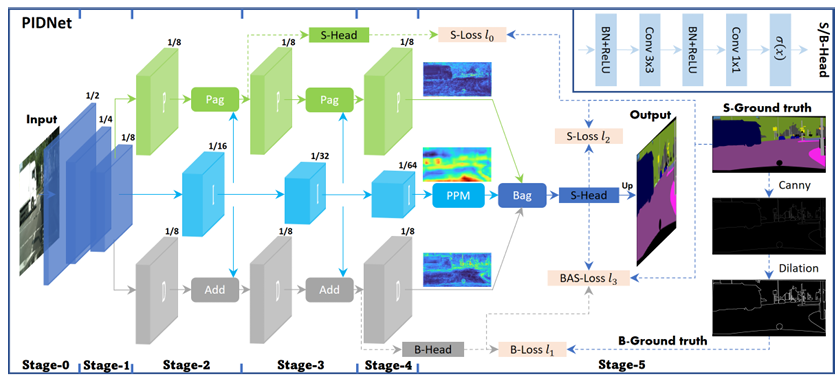
\includegraphics[width=1\linewidth]{image/general/PIDNET.png}
	\caption{An overview of the basic architecture of our proposed Proportional-Integral-Derivative Network (PIDNet)}
	\label{fig:PIDNET_image}
\end{figure}

\begin{multicols}{2}
\subsubsection{2b Efficient segmentation framework}
To establish real-time capability baselines, we employed PIDNet-S - a streamlined architecture that mimics proportional-integral-derivative control mechanisms through three parallel branches. These branches explicitly manage high-frequency details, mid-level structures, and low-level spatial relationships respectively. The model was similarly initialized with ImageNet weights and trained and evaluated on urban scenes.





\subsubsection{PIDNet architecture details}
The core PIDNet architecture \cite{pidnet2023} consists of three branches (Figure \ref{fig:PIDNET_image})
\begin{itemize}
	\item \textbf{Proportional (P) branch}: Processes full-resolution inputs using shallow layers to preserve spatial precision. Contains edge-aware convolutions for sharp boundary detection.
	\item \textbf{Integral (I) branch}: Leverages deep layers with dilated convolutions and spatial pooling to capture multi-scale context. Integrates a Semantic Guidance Module (SGM) to filter low-level noise.
	\item \textbf{Derivative (D) branch}: Computes high-frequency feature discrepancies between adjacent stages using depthwise separable convolutions. Acts as a boundary corrector by amplifying transitional regions.
\end{itemize}
The branches are fused through a \textit{Three-Way Attention Fusion (TWAF)} module that dynamically combines features using spatial and channel attention weights.
 
\subsection{3a Domain adaptation }
\label{subsec:domain_shift}
We investigated cross-domain generalization by evaluating our urban-trained PIDNet-S on the LoveDA-rural dataset without fine-tuning. This experimental design isolates the domain shift problem between man-made urban environments (characterized by geometric regularity and dense infrastructure) and rural landscapes (featuring organic shapes, sparse structures, and varied terrain).
(Figure \ref{fig:dataset_mix})
\\

\begin{figure}[H]
	\centering
	\begin{minipage}{0.48\linewidth}
		\centering
		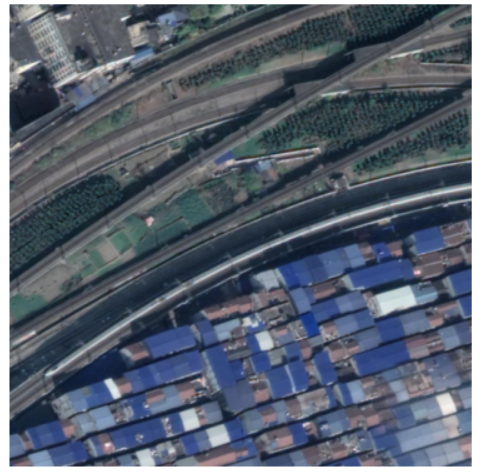
\includegraphics[width=1\linewidth]{image/urban_2.png}

	\end{minipage}
	\begin{minipage}{0.48\linewidth}
		\centering
		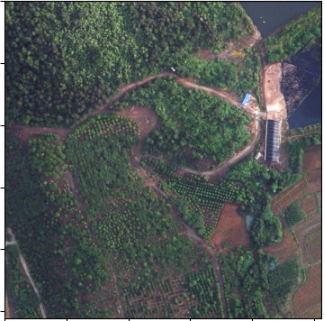
\includegraphics[width=1\linewidth]{image/rural_2.png}

	\end{minipage}
	\caption{Example of urban image (left) and rural image (right)}
	\label{fig:dataset_mix}

	\hfill
	\\


\end{figure}



\subsubsection{Domain adaptation challenges}
The performance degradation observed could be caused by:  
\begin{itemize}
\item1) \textbf{Object scale variance}: Urban structures maintain relatively consistent scales, while rural elements exhibit greater size variability (trees, water bodies)  
\item2) \textbf{Contextual dependencies}: Urban scene semantics rely on positional relationships (e.g., roads between buildings), whereas rural contexts depend more on texture and color patterns  
\item3) \textbf{Surface color distribution}: Artificial materials dominate urban areas (concrete, glass) (Figure \ref{fig:dataset_mix}), contrasting with natural materials (soil, vegetation) prevalent in rural regions.
\end{itemize}
This analysis motivates subsequent domain adaptation strategies to bridge the feature distribution gap between structurally distinct environments.

\begin{figure}[H]
	\centering
	\begin{minipage}{0.48\linewidth}
		\centering
		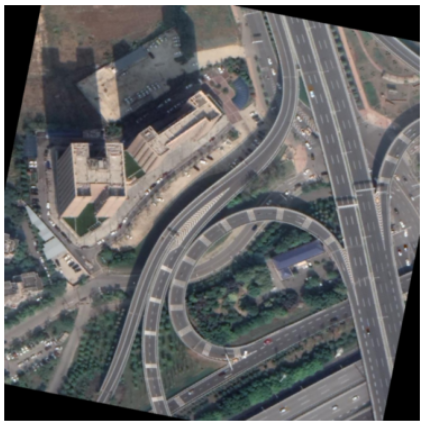
\includegraphics[width=1\linewidth]{image/aug/4_aug1+urban.png}

		
	\end{minipage}
	\begin{minipage}{0.48\linewidth}
		\centering
		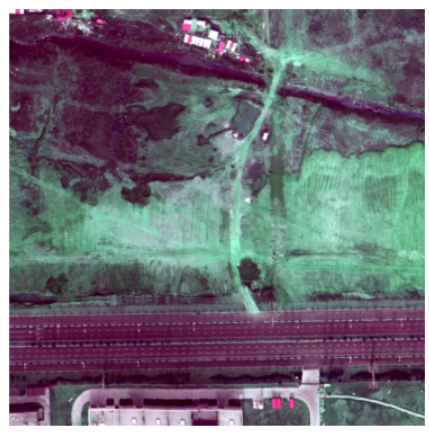
\includegraphics[width=1\linewidth]{image/aug/3_aug2.png}
		
		
	\end{minipage}
	\caption{The left image is modified by augmentation A1, while the right image is modified by augmentation A2.}
	
	\label{fig:data_aug}

\end{figure}


		\subsection{3b Data augmentation}
		Data augmentation was used to improve the model's generalization capability by increasing the diversity of the training data. Two augmentation strategies were applied during training with a probability of 0.5:
		(Figure \ref{fig:data_aug})
		
		
		\begin{itemize}
			\item \textbf{A1}: Geometric transforms (horizontal/vertical flips, 30° rotation)
			\item \textbf{A2}: Photometric transforms (ColorJitter, GaussianBlur)
		\end{itemize}
		Photometric augmentations were more effective because they help the model become invariant to changes in lighting and color, which are common differences between the urban and rural domains.
		
\subsection{Unsupervised domain adaptation}  
 
This method aligns domains through adversarial training on segmentation outputs \cite{tsai2018learning}, comprising three phases:  

\paragraph{Phase 1: Source domain training}  
The segmentation network $G$ processes source images $I_s$ to produce softmax probability maps:  
\begin{equation}  
	P_s = {softmax}(G(I_s)) \in {R}^{C \times W \times H}  
\end{equation}  
where $C$ denotes semantic classes. Training uses standard cross-entropy loss with source labels $Y_s$.  



\paragraph{Phase 2: Adversarial alignment}  
The segmentation network now receives gradients to confuse $D$ by:  
\begin{itemize}  
	\item Maximizing discriminator uncertainty on $P_t$ (domain label 1)
	\item Enforcing similar output distributions $P_s \approx P_t$  

\end{itemize}  

\paragraph{Phase 3: Discriminator training}  
A fully-convolutional discriminator $D$ learns to distinguish:  
\begin{itemize}  
	\item Source softmax outputs $P_s$ (domain label 1)  
	\item Target softmax outputs $P_t = {softmax}(G(I_t))$ (domain label 0)  
\end{itemize}  


This single-stage approach achieves domain invariance by directly matching the structured output distributions rather than intermediate features.  
\begin{figure}[H]
	\centering
	\begin{minipage}{0.48\linewidth}
		\centering
		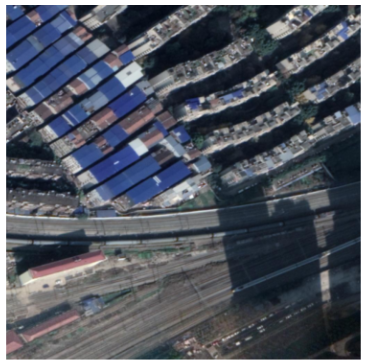
\includegraphics[width=1\linewidth]{image/dacs_source2.png}

		
	\end{minipage}
	\begin{minipage}{0.48\linewidth}
		\centering
		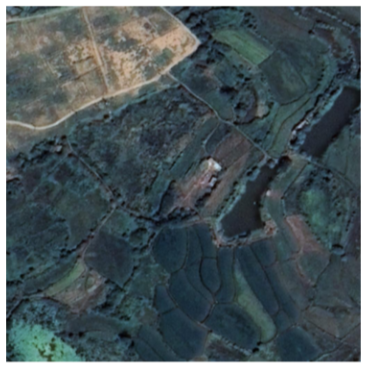
\includegraphics[width=1\linewidth]{image/dacs_target2.png}

	\end{minipage}
	% \caption{}

	\hfill
	\\
	\begin{minipage}{0.48\linewidth}
		\centering
		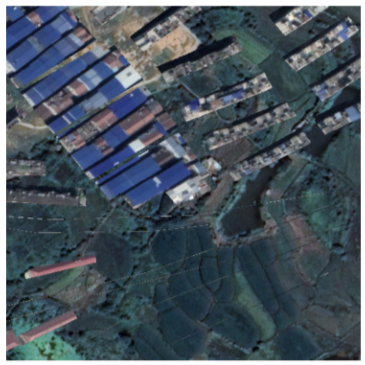
\includegraphics[width=1\linewidth]{image/dacs_mixed2.png}
		
	\end{minipage}


	\caption{(top left) urban sample, (top right) rural sample, (bottom) hybrid sample}
	\label{fig:DACS_image_result}

\end{figure}


	\subsubsection{4b DACS}
	
	Domain Adaptation (Figure \ref{fig:DACS_image}) via Cross-domain Mixed Sampling (DACS) \cite{tranheden2021dacs} addresses unsupervised domain adaptation (UDA) by blending data from the source and target domains through class-level mixing. The main aspects of DACS are:
	
	\begin{itemize}
		\item \textbf{Augmented training samples:} 
		DACS creates hybrid samples by combining (Figure \ref{fig:DACS_image_result}):
		\begin{itemize}
			\item A source domain image, which comes with ground-truth labels.
			\item A target domain image, which has pseudo-labels generated by the model.
		\end{itemize}
		During this process, a subset of classes is selected from the source image using its semantic map, and the corresponding pixels are pasted onto the target image.
		
		\item \textbf{Composite label generation:}
		The labels for the mixed image are produced by merging:
		\begin{itemize}
			\item Ground-truth labels from the source image.
			\item Pseudo-labels predicted for the target image.
		\end{itemize}
		This ensures that the model is trained on hybrid data containing both reliable source annotations and target pseudo-labels, encouraging feature invariance across domains.
		

		\item \textbf{Training loss:} 
		The overall loss combines:
		\begin{itemize}
			\item Supervised learning on the source domain data.
			\item Consistency regularization on the mixed-domain samples.
		\end{itemize}
		Importantly, this does not require any annotations from the target domain.
		

	\end{itemize}

	\begin{figure}[H]
		\centering
		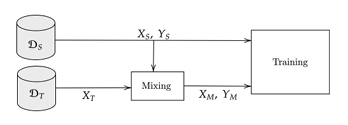
\includegraphics[width=1\linewidth]{image/general/DACS_structure.png}
		\caption{  Diagram showing DACS. The images X\textsubscript{S} and X\textsubscript{T} are
		mixed together, using Y\textsubscript{S} for the labels of X\textsubscript{S}, instead of a pre
	   dicted semantic map to determine the binary mask. The segmenta
	   tion network is then trained on both batches of augmented images
		and images from the source dataset.}
		\label{fig:DACS_image}
	\end{figure}	
	
		
		\subsubsection{Extensions}
		We explored three alternative real-time semantic segmentation architectures:
		\begin{itemize}
			\item \textbf{BiSeNetV1} \cite{yu2018bisenet}: Employs a dual-path design with a \textit{spatial path} (high-resolution stream for fine details) and a \textit{context path} (fast downsampling with global average pooling for long-range dependencies). The features are fused using a specialized Feature Fusion Module (FFM).
			\item \textbf{LinkNet} \cite{chaurasia2017linknet}: Uses a lightweight encoder-decoder structure with residual skip connections. The encoder reduces spatial dimensions through cascaded convolutional blocks, while the decoder employs transposed convolutions for upsampling, with direct additive links between corresponding encoder-decoder layers.
			\item \textbf{STDC n} \cite{fan2021rethinking}: Features a Short-Term Dense Concatenate backbone that progressively aggregates multi-scale features through dense connections in early stages, followed by a Context Path with Attention Refinement Modules (ARMs) to enhance contextual awareness.
		\end{itemize}
		These models emphasize distinct architectural strategies: BiSeNetV1's parallel multi-resolution processing, LinkNet's symmetrical skip connections, and STDCNet's dense feature aggregation.
		

		\begin{figure}[H]  

			\centering
			\begin{minipage}{1\linewidth}
				\centering
				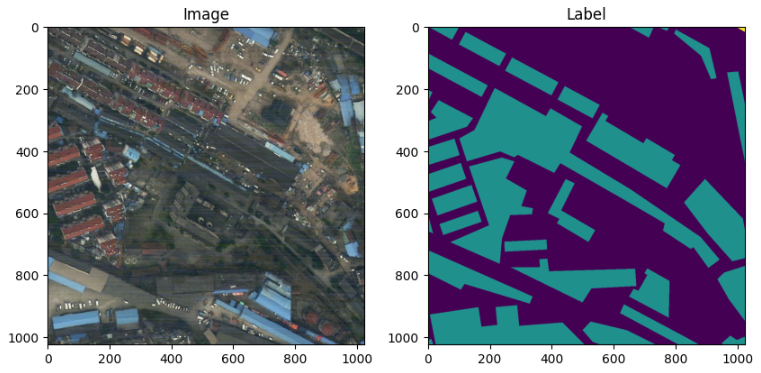
\includegraphics[width=1\linewidth]{image/urban+mask4.png}
				
			\end{minipage}
			\begin{minipage}{1\linewidth}
				\centering
				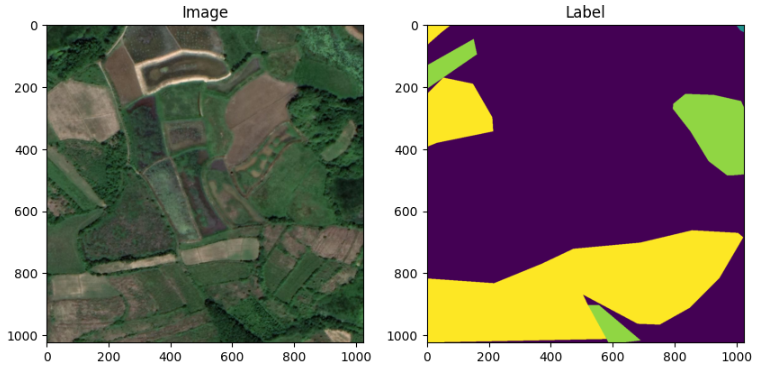
\includegraphics[width=1\linewidth]{image/rural+mask4.png}
				
			\end{minipage}
			\caption{Class distribution similarities between urban (top) and rural (bottom) domains in LoveDA: the background class dominates both domains.}  
			\label{fig:class_eug}  

		\end{figure}



		\section{Experimental results}

		\subsection{LoveDA dataset}  
		The LoveDA dataset \cite{loveda2021} is a high-resolution (0.3 m) remote sensing dataset designed for domain-adaptive semantic segmentation in urban and rural environments. It contains 5,987 images across three Chinese cities (Nanjing, Changzhou, Wuhan), annotated with seven classes: *background*, *building*, *road*, *water*, *barren*, *forest*, and *agriculture*. The dataset is explicitly divided into urban (2,522 images) and rural (3,465 images) domains to study domain shift challenges.  
		
		Key characteristics of LoveDA include:  
		\begin{itemize}  
			\item \textbf{Multi-scale objects}: Urban scenes feature densely packed buildings and structured roads, while rural areas contain scattered agricultural plots and irregular water bodies. Buildings in urban regions exhibit larger size variance compared to rural regions (Figure \ref{fig:dataset_rural_image1}).  
			\item \textbf{Complex backgrounds}: The *background* class dominates both domains (Figure \ref{fig:class_eug}), encompassing diverse elements like vehicles and undeveloped land, which introduces high intra-class variance.  
			\item \textbf{Domain shift}: Urban and rural domains exhibit divergent class distributions (e.g., urban has 32\% buildings vs. rural’s 8\%) and spectral properties (lower variance in rural areas due to homogeneous landscapes)(Figure \ref{fig:class_div}).  
		\end{itemize}  
		
		\begin{figure}[H]  

			\centering
			\begin{minipage}{1\linewidth}
				\centering
				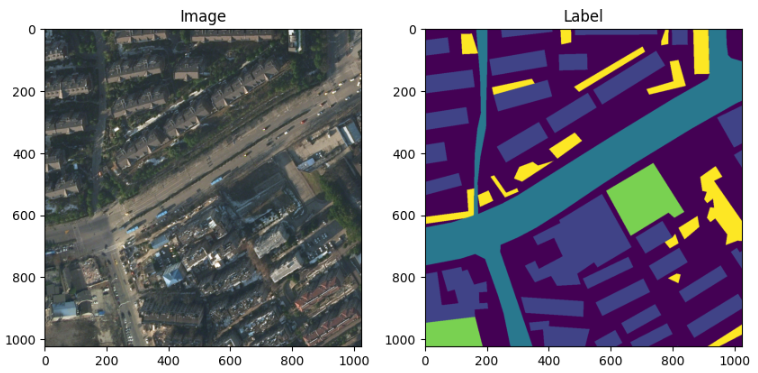
\includegraphics[width=1\linewidth]{image/urban+mask2.png}
				
			\end{minipage}
			\begin{minipage}{1\linewidth}
				\centering
				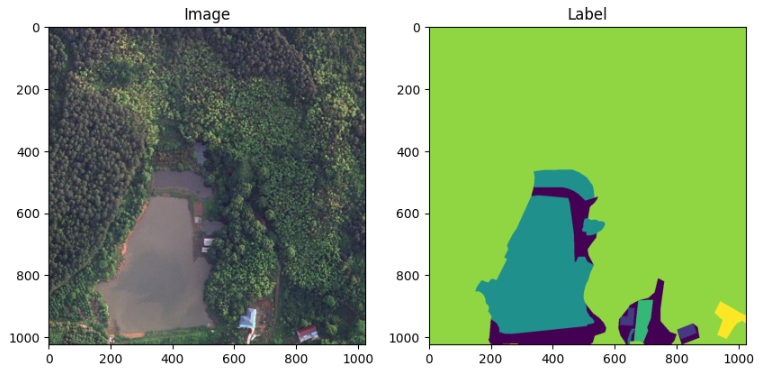
\includegraphics[width=1\linewidth]{image/rural+mask5.png}
				
			\end{minipage}
			\caption{Class distribution diversity between urban (top) and rural (bottom) domains in LoveDA.}  
			\label{fig:class_div}  

		\end{figure}


		\subsection{Performance on source domain}
		Table \ref{tab:urban} shows the performance of DeepLabV2 and PIDNet-S on the LoveDA-urban dataset (source domain). PIDNet-S, designed for real-time performance, achieved a significantly higher mIoU than DeepLabV2 while also providing latency, FLOPs, and parameter count.


		\begin{table}[H]
			\centering
			\renewcommand{\arraystretch}{1.2} % Aumenta lo spazio tra le righe per leggibilità
			\setlength{\tabcolsep}{6pt} % Regola la spaziatura tra colonne
			
			\resizebox{\linewidth}{!}{ % Ridimensiona automaticamente la tabella alla larghezza della pagina
				\begin{tabular}{|l|c|c|c|c|}
					\hline
					Model & mIoU (\%) & Latency (ms) & FLOPs & Params \\ \hline
					DeepLabV2 & 33.41 & 13.42 & 11.535G & 62.231M \\ \hline
					PIDNet-S & 48.67 & 288.70 & 6.35G & 7.72M \\ \hline
				\end{tabular}
			}
			\caption{Performance comparison of different hyperparameter tuning.}
			\label{tab:urban}
		\end{table}




		\subsection{Domain shift evaluation}
		\small
		Table \ref{tab:shift} quantifies the domain shift from LoveDA-urban to LoveDA-rural. The baseline PIDNet-S model, trained on urban data, experienced a significant performance drop when tested on rural data. Data augmentations (A1 and A2) improved the mIoU, with A2 (photometric transforms) being the most effective. Adversarial training and DACS further mitigated the domain shift, achieving similar performance.
		
	
		\begin{figure}[H]
			\centering
			\begin{minipage}{0.8\linewidth}
				\centering
				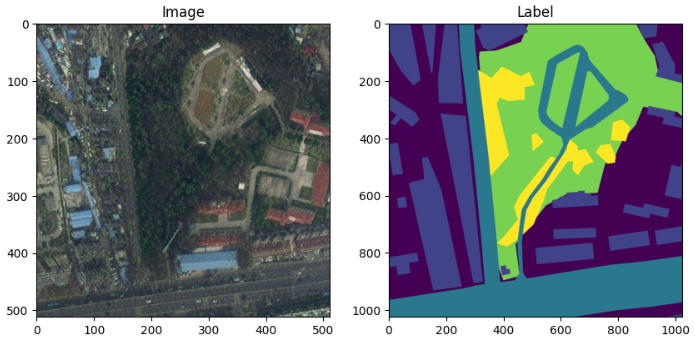
\includegraphics[width=1\linewidth]{image/nst/urban+mask2.png}

				
			\end{minipage}
			\begin{minipage}{0.8\linewidth}
				\centering
				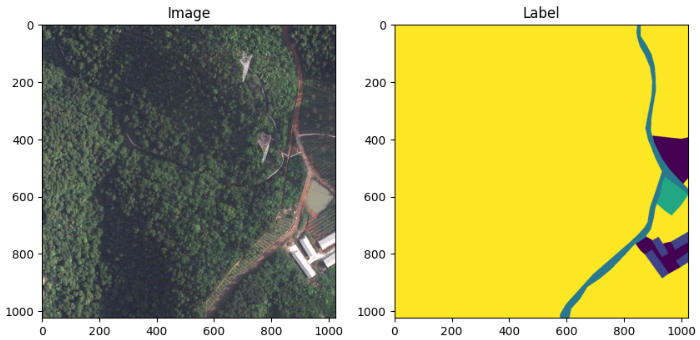
\includegraphics[width=1\linewidth]{image/nst/rural+mask2.png}
				
			\end{minipage}

			% \hfill
			\begin{minipage}{0.8\linewidth}
				\centering
				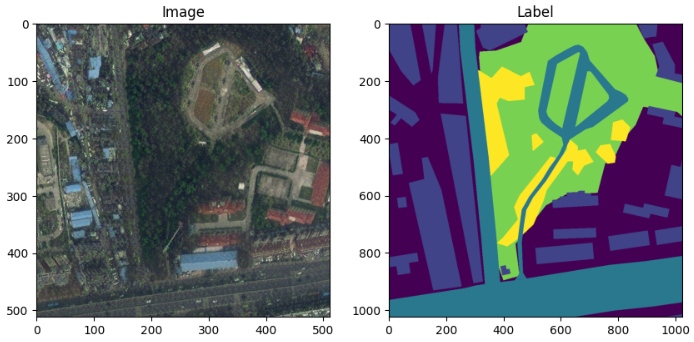
\includegraphics[width=1\linewidth]{image/nst/mixed+mask2.png}

			\end{minipage}


			\caption{urban image }
			\label{fig:transfer}

		\end{figure}



		\subsection{Extensions}
		\justifying
		Table \ref{tab:extensions} presents the results of the extensions on the LoveDA-rural dataset. Style transfer preprocessing improved the mIoU slightly compared to the baseline but was less effective than data augmentation or domain adaptation techniques. BiSeNetV1 and LinkNet showed competitive performance, with BiSeNetV1 outperforming PIDNet-S on the target domain.
		

		\begin{table}[H]
			\centering
			\renewcommand{\arraystretch}{1.2} % Aumenta lo spazio tra le righe per leggibilità
			\setlength{\tabcolsep}{14pt} % Regola la spaziatura tra colonne
			
			\resizebox{\linewidth}{!}{ % Ridimensiona automaticamente la tabella alla larghezza della pagina
			\begin{tabular}{|l|c|}
				\hline
				Model & mIoU (\%) \\ \hline
				PIDNet + Style Transfer (Figure \ref{fig:transfer}) & 25.46 \\ \hline
				BiSeNetV1 & 32.21 \\ \hline
				LinkNet & 30.43 \\ \hline
				BiSeNet Stdc & 34.10 \\ \hline
			\end{tabular}
			}
			\caption{Performance comparison of different models on rural images.}
			\label{tab:extensions}

		\end{table}


        \subsubsection{Hyperparameter tuning Rresults and analysis}
        \justifying
        Table \ref{tab:hyperparameters} presents the results of hyperparameter tuning experiments conducted on the LoveDA-rural dataset. The default configuration (batch size = 16, learning rate = \(10^{-4}\)) achieved the highest validation mIoU of 30.63\%. Smaller batch sizes (2, 8) resulted in worse performance, likely due to instability in training and poor gradient estimation. Increasing the learning rate to \(10^{-3}\) degraded performance, probably because of convergence issues. The adaptive lambda adjustment also did not improve results, showing limited generalization benefits.
        


		\begin{table}[H]
			\centering
			\renewcommand{\arraystretch}{1.4} % Aumenta lo spazio tra le righe per leggibilità
			\setlength{\tabcolsep}{6pt} % Regola la spaziatura tra colonne
			
			\resizebox{\linewidth}{!}{%
			\begin{tabular}{|l|c|}
				\hline
				Configuration & Best Validation mIoU (\%) \\ \hline
				Batch Size = 16, LR = \(10^{-4}\) (Default)  & 30.63 \\ \hline
				Batch Size = 2, LR = \(10^{-4}\)  & 15.00 \\ \hline
				Batch Size = 8, LR = \(10^{-4}\)  & 16.59 \\ \hline
				Batch Size = 16, LR = \(10^{-3}\)  & 19.09 \\ \hline
				Batch Size = 16, Adaptive Lambda  & 18.26 \\ \hline
			\end{tabular}
			}
			\caption{Performance comparison of different models on urban images.}
			\label{tab:hyperparameters}

		\end{table}



        Smaller batch sizes (2, 8) resulted in significantly lower performance, likely due to higher gradient noise and instability in training, leading to suboptimal convergence. A higher learning rate (\(10^{-3}\)) caused a decrease in mIoU, probably due to overshooting during optimization, preventing the model from reaching a good local minimum. The introduction of an adaptive lambda strategy, while theoretically beneficial for balancing losses dynamically, did not improve the results, possibly due to inadequate adaptation to the dataset characteristics or suboptimal parameter tuning.

	\end{multicols}
	\begin{table}[H]
		\centering
		\renewcommand{\arraystretch}{1.2} % Aumenta lo spazio tra le righe per leggibilità
		\setlength{\tabcolsep}{10pt} % Regola la spaziatura tra colonne
		

		\resizebox{\linewidth}{!}{ % Ridimensiona automaticamente la tabella alla larghezza della pagina
				\begin{tabular}{|l|c|c|c|c|c|c|c|}
					\hline
					Model & Road & Building & Water & Barren & Forest & Agric. & mIoU \\ \hline
					PIDNet & 16.34 & 23.99 & 35.46 & 3.12 & 8.83 & 31.82 & 23.98 \\ \hline
					+ A1 & 29.33 & 40.77 & 36.71 & 9.17 & 9.53 & 33.13 & 29.91 \\ \hline
					+ A2 & 31.41 & 38.37 & 31.33 & 10.26 & 15.10 & 37.51 & 30.80 \\ \hline
					+ A1 + A2 & 27.92 & 32.97 & 33.98 & 10.50 & 10.69 & 37.45 & 29.35 \\ \hline
					+ Adv. & 0.36 & 13.41 & 32.72 & 8.28 & 49.73 & 12.26 & 30.59 \\ \hline
					+ DACS & 31.32 & 36.60 & 42.70 & 4.49 & 2.70 & 40.60 & 30.63 \\ \hline
				\end{tabular}
		}
		\label{tab:shift}
		\caption{Performance comparison of different version of aumented dataset.}


	\end{table}

	\begin{multicols}{2}





        \subsubsection{Loss function comparison}
        \justifying
        Table \ref{tab:loss_functions} presents the results of different loss functions evaluated on the LoveDA-rural dataset. The default configuration utilized OhemCrossEntropy with the DACS loss formulation, achieving the highest validation mIoU of 30.63\%. 
        Boundary loss resulted in the worst performance, with a validation mIoU of 8.50\% and a considerably higher loss value of 11.1707. This high loss value points to issues with gradient propagation, potentially caused by boundary loss not being as effective at focusing on difficult regions. The model likely failed to effectively learn from the more complex areas of the image, resulting in low accuracy and unstable training.
        CrossEntropy loss improved upon boundary loss, with a validation mIoU of 24.59\% and a loss value of 0.8962. While the loss value is lower than that of boundary loss, the performance still lags behind the default OhemCrossEntropy + DACS setup. The absence of Online Hard Example Mining (Ohem), which helps prevent bias towards background pixels, could explain this drop in mIoU. The model might have focused on easier examples and ignored the more difficult ones, leading to a suboptimal performance.
        Dice loss performed slightly worse than CrossEntropy loss, achieving a validation mIoU of 22.66\% with a corresponding loss value of 0.6475. Dice loss is typically used to address class imbalance, but in this case, it did not outperform the default setup. The lack of an explicit mechanism to focus on difficult or hard-to-learn pixels, which Ohem provides, might explain why Dice loss was not as effective in this context. While the lower loss value is a positive indicator, it does not directly translate to improved mIoU.

        
        \begin{table}[H]
			\centering
			\renewcommand{\arraystretch}{1.4} % Aumenta lo spazio tra le righe per leggibilità
			\setlength{\tabcolsep}{6pt} % Regola la spaziatura tra colonne
			
			\resizebox{\linewidth}{!}{%
            \begin{tabular}{|l|c|c|}
                \hline
                Loss Function & Validation mIoU (\%) & Loss Value \\ \hline
                OhemCrossEntropy + DACS (Default) & 30.63 & 0.7993 \\ \hline
                Boundary Loss & 8.50 & 11.1707 \\ \hline
                CrossEntropy Loss & 24.59 & 0.8962 \\ \hline
                Dice Loss & 22.66 & 0.6475 \\ \hline
            \end{tabular}
            }
			\caption{Performance comparison of different loss functions.}
			\label{tab:loss_functions}

		\end{table}


		\subsection{Comparison with original UDA paper results}
		Table \ref{tab:uda_comparison} compares our domain adaptation results with those reported in the original DACS paper \cite{tranheden2021dacs} and LoveDA benchmarks \cite{loveda2021}. While DACS achieved 39.10\% mIoU on LoveDA-rural in the original implementation, our PIDNet-S adaptation reached only 30.63\%. Similarly, adversarial training underperformed compared to Tsai et al. \cite{tsai2018learning} (30.59\% vs. 35.20\%). Three key factors explain these differences:
		
		\begin{itemize}
			\item \textbf{Model architecture}: The original DACS paper used DeepLabV2 with ResNet-101, which has significantly higher capacity (44.5M params) compared to our real-time PIDNet-S (7.72M params). This architectural difference directly impacts feature representation power.
			\item \textbf{Training constraints}: Our experiments used a fixed 20-epoch training schedule to maintain real-time deployment capabilities, whereas the original works employed longer training (50+ epochs) with extensive hyperparameter tuning.
			\item \textbf{Latency-Accuracy trade-off}: PIDNet-S prioritizes inference speed (288ms) over pure accuracy, while DeepLabV2-based implementations ignore latency constraints (typically 1,000ms).
		\end{itemize}
		
		\justifying
		These results highlight the inherent challenge of balancing domain adaptation performance with real-time requirements—a critical consideration for edge deployment scenarios.
		

		\begin{table}[H]
			\centering
			\renewcommand{\arraystretch}{1.4} % Aumenta lo spazio tra le righe per leggibilità
			\setlength{\tabcolsep}{6pt} % Regola la spaziatura tra colonne
			
			\resizebox{\linewidth}{!}{%
			\begin{tabular}{|l|l|c|c|}
				\hline
				Method & Model & mIoU (\%) & Latency (ms) \\ \hline
				DACS (Original) \cite{tranheden2021dacs} & DeepLabV2 + ResNet-101 & 39.10 & 1,200 \\ \hline
				DACS (Ours) & PIDNet-S & 30.63 & 288 \\ \hline
				Adv. Training (Original) \cite{tsai2018learning} & DeepLabV2 + VGG16 & 35.20 & 850 \\ \hline
				Adv. Training (Ours) & PIDNet-S & 30.59 & 288 \\ \hline
			\end{tabular}%
		}
			\caption{Performance comparison with original UDA paper results.}
			\label{tab:uda_comparison}

		\end{table}



		\section{Conclusion}
		\justifying


		This study highlights the effectiveness of PIDNet for real-time semantic segmentation, achieving a strong performance on the LoveDA-urban dataset (288ms latency, 48.67\% mIoU). However, the impact of domain shift, as observed on LoveDA-rural (23.98\% mIoU), underscores the challenges of applying segmentation models across divergent environments. Among the evaluated mitigation strategies, photometric data augmentation (A2) showed the most consistent improvement (+6.82\% mIoU), while adversarial training and DACS offered moderate yet comparable gains (+6.61\% and +6.65\% mIoU, respectively). Despite these advancements, the trade-off between accuracy and computational efficiency remains a key limitation, particularly in edge computing scenarios. 
		\\
		Our experiments demonstrate that while PIDNet excels in maintaining real-time capabilities, alternative architectures like BiSeNetV1 can surpass it in domain-adaptive accuracy, at a slight cost to speed. These findings suggest that a hybrid approach, integrating the efficiency of PIDNet with enhanced feature representation techniques from other models, could be a promising direction.
		Future research could focus on:

		\begin{enumerate}
			\item \textbf {Hybrid Adaptation Strategies}: Combining DACS with adversarial training or exploring ensemble techniques to synergize their strengths.
			\item \textbf {Optimized Style Transfer Pipelines}: Refining preprocessing steps to reduce the spectral and textural differences between domains.
			\item \textbf {Domain-Specific Fine-Tuning}: Introducing lightweight domain-specific adaptations during deployment to address localized variations.
			\item \textbf {Longer Training Regimes}: Exploring optimized training schedules that balance performance improvements with real-time constraints.
		\end{enumerate}
		
		Ultimately, this work provides a foundation for advancing domain-adaptive real-time semantic segmentation, offering practical insights for deploying robust models in dynamic, real-world environments where domain variability is unavoidable.
		

		
	\end{multicols}
	
	\bibliographystyle{ieeetran}
	\bibliography{references}
	
\end{document}